\chapter{Biomechanik}

Die Biomechanik ist eine interdisziplinäre Wissenschaft, die den Bewegungsapparat biologischer Systeme (menschlich, tierisch, künstlich) untersucht. Biomechanik wird z.B. in der Diagnose von Erkrankungen des menschlichen Bewegungsapparates, bei Gelenkersatz (z.B. künstliches Hüftgelenk) oder Prothesen eingesetzt. Dabei wird zwischen der Kinematik und der Kinetik unterschieden. Die Kinematik beschreibt die Bewegung von Punkten im Raum, also z.B. die Gelenkwinkel, Winkelgeschwindigkeiten oder Winkelbeschleunigung. Die Kinetik die Einwirkung von Kräften und Momenten auf einen Körper.

In der Biomechanik wird ein biomechanisches Modell verwendet, um die Bewegungen der Marker mit der zugrundeliegenden Anatomie in Relation zu bringen. Im Rigid Body Model sind starre Segmente (Hand, Unterarm, Oberarm usw.) durch ideale Kugelgelenke verbunden. Dadurch kann das Gelenkkoordinatensystem bestimmt werden. Dazu wird am Körper drei Marker pro Segement an Stellen mit geringen Hautverschiebungen positioniert. Dann kann z.B. das Koordinatensystem für das Ellenbogengelenk bestimmt werden (siehe Abbildung \ref{fig:ellenbogen}).

In der Kinetik müssen die externen Kräfte und Momente welche auf den Körper wirken, durch interne Kräfte und Momente kompensiert werden. Externe Kräfte sind Gewichtskraft und zusätzliche durch Randbedingungen aufgebrachte Kräfte und können gemessen (z.B. Federwaage, Biegebalken, Kraftmessplatten oder Isokineten) oder berechnet werden.

\begin{figure}[h!]
	\centering
	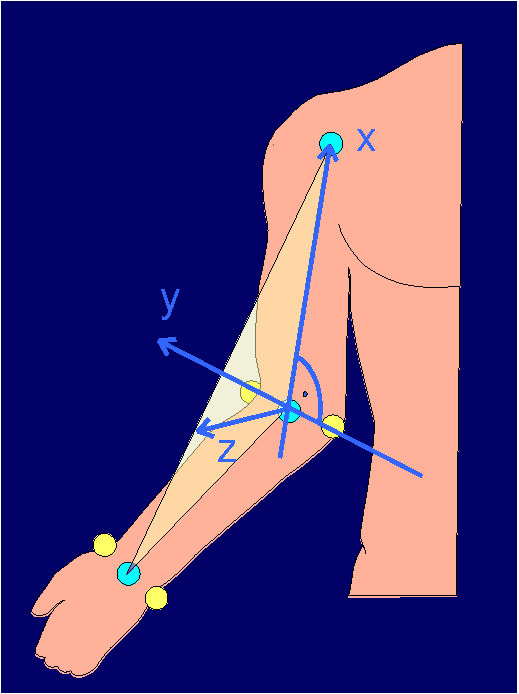
\includegraphics[width=0.4\linewidth]{fig/ellenbogen}
	\caption{Koordinatensystem des Ellenbogens}
	\label{fig:ellenbogen}
\end{figure}